\documentclass[12pt]{article}
\usepackage{amsthm}
\usepackage{amsmath}
\usepackage{graphicx}


% collectivised from: https://www.overleaf.com/learn/latex/Theorems_and_proofs#Theorem_styles
\theoremstyle{definition}
\newtheorem{definition}{Definition}[section]

\theoremstyle{remark}
\newtheorem*{remark}{Remark}
\newtheorem{theorem}{Theorem}[section]
\newtheorem{lemma}[theorem]{Lemma}
%
\begin{document}
    

Let $G:= (V, E)$ be a bridgless undirected cubic planar graph.
\begin{lemma}
    If $G$ is cubic, then $|V|$ is even.
\end{lemma}

\begin{proof}
    $2|E| = \sum_{v \in V} d(v) = 3|V| $ \\
    As $|E|$ must be integer, it follows that we must be able o divide $|V|$ by 2.
\end{proof}

\begin{lemma}
    If $G$ is cubic, planar and bridgless, then $G$ has a chromatic index of 3. 
\end{lemma}


Consider the graph $G':= (V', E')$, obtained from $G$ by removing an edge $xy$, adding a vertex $z$, and adding edges $xz$ and $yz$. 
\begin{lemma}
    $G'$ has a chromatic index of 4.
\end{lemma}

\begin{proof}
    As $\Delta(G') = 3$; we prove the $\chi'(G') \le 4$ thanks to Vizing's theorem.\\
    Now consider a matching $M$ of the edges of $E'$. as $|V'| = |V|+1$ is odd, each matching can cover at most $|V|$ vertices,
    so it can at most contains $\tfrac{|V|}{2}$ edges. However, we have $|E'| = \tfrac{3}{2} |V| + 1$ edges, so we must have $\chi'(G') \ge 4$.
\end{proof}






\newpage
\section{On-a-grid graphs}

We know that the concept of directions in a unit-square graphs has proved quite useful. For instance, we know that for $C_4$; all the squares must have their
neighbours in adjacent directions; for a $C_5$; exactly one square has it's neighboursin opposite directions, etc. \\
We propose here a new tool to these particular graphs. It will prove rather useful later to prove a large number of statements. 

\begin{definition} [On-a-grid]
    A graph $G$ is said on-a-grid if it is represented such that $\forall e_1, e_2 \in E(G)$, $e_1$ and $e_2$ are either parallels or perpendicular, and no edge is represented including an other.
    Moreover, the length of all the edges is a integer. 
\end{definition}

\begin{figure}[h]
    \centering
    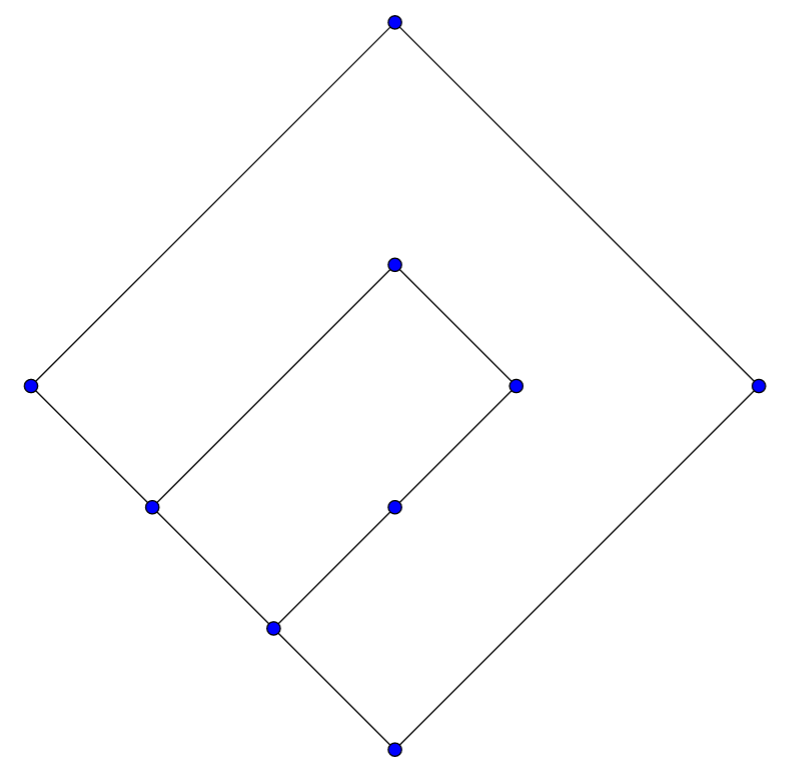
\includegraphics[scale=0.2]{tex_images/on_a_grid_g1.png}
    \caption{The graph $G$ is on-a-grid.}
\end{figure}

\begin{remark}
    There is no ambiguity or "hidden" edges; so, for instance, only $10$ edges in Fig. 1.
\end{remark}

\begin{lemma}
    All on-a-grid graphs are triangle-free.
\end{lemma}

\begin{proof}
    A non-degenerate triangle can't have only parallel or perpendicular edges.
\end{proof}

There exists two special lines in the representation of a on-a-grid graph: those such that every edge is parallel to one of them.
These are called the \textit{directions of the grid}.
We will only consider the case where they are represented with a $\tfrac{\pi}{4}$ angle with regard to the usual cartesian system (see Fig.1) as it will be more convenient for the future applications.

\begin{definition}[RL, LR lines]
    We refer to the \textit{directions of the grid} as LR and RL: LR is the one going from down Left to up Right; RL is the other one. 
\end{definition}

RL and LR lines will be useful later to consider "layers" of vertices to generate an algorithm to pass from a representation to another
% OR just from squares to on-a-grid, who knows.

\begin{lemma}
    If $G$ is on-a-grid, $\Delta(G) \le 4$.
\end{lemma}

\begin{proof}
    Trivial.
    %Suppose by contradiction that $G$ is on a grid with a vertex $v$ such that $d(v) \ge 5$. \\
    %Call $e_1, .. e_5$ five distinct edges of $G$ containing $v$. \\
    %As every edge is parallel to one of RL or LR it means at least three of the $e_1, .. e_5$ are parallel; suppose it is $e_1, e_2$ and $e_3$.\\
\end{proof}

\begin{definition}[DL, DR, UL, UR directions]
    Let $xy$ be an edge of $G$ we say that $xy$ is in the UR (Up-Right) direction if: $xy$ is parallel to LR and $y$ is higher on the plane than $x$.\\
    We have analogous definitions for UL, DR and  DL. 
\end{definition}

\begin{remark}
    if $xy$ is in UR direction, then $yx$ is in DL direction.
\end{remark}

\begin{definition}[upper vertex, upper edge]
    We say that $y$ is a vertex upper than $x$ if there exists a path $xv_1-v_ky$ possibly trivial such that every edge of the path is in direction UL or UR. 
    An edge is upper than a vertex $v$ if it contains a vertex upper than $v$.
\end{definition}

We have analogous definition for lower, righter and lefter.



\subsection{From square corner intersection graphs to on-a-grid representation }

\begin{definition}[$P(UR)$]
    Let $P$ be a path in $G$. $P(UR)$ is the number of UR connection in $P$.
\end{definition}

\begin{definition}[on the same RL diagonal] %remark: it could use a lower/higher version. Think of a last layer
    Let $G$ be an intersection graph of a corner square family. Let $x, y$ be two squares of $G$. $x$ and $y$ are said to be on the same RL diagonal
    if the smallest path $P$ from $x$ to $y$ using only UL, UR and DL connections have $P(UR) = P(DL)$. 
\end{definition}

See on the Fig. 2 for instance: A, D and F are on the same RL diagonal. Although there exist a path from F to D in 3 UR and 1 DL connection, the smallest one is the trivial FD. \\
We can observe that, if this definition is clear when the squares share a UL connection, it is also true when they are disjoint; in this example, I and G are on the same RL diagonal.\\
We have an analogous definition for squares on the same LR diagonal; here: F, E, I, H for instance.

\begin{figure}[h]
    \centering
    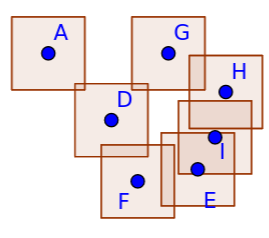
\includegraphics[scale=0.3]{tex_images/same_diagonals.png}
    \caption{Example of corner intersection graph.}
\end{figure}

\begin{definition}[number of diagonals]
    The number of RL diagonals of a square corner intersection graph $G$ is the number regroupements you must make of squares that are on the same RL diagonal in order to take in account every square.

\end{definition}

For instance in Fig. 2 we have 4 RL diagonals, the regroupements being: $\{(A, D, F); (E); (I, G); (H) \}$.\\
We have an analogous definition for the number of LR diagonals; here, there are only 3.

\begin{definition}[order on diagonals]
    Let two RL distinct diagonals $D := \{d_1, d_2, ... d_k \} $ and $E:= \{e_1, ... e_l\}$.   \\
    We say that $D<E$ if:  
    $$\forall d_i, e_j, d_{RL}(d_i, e_j) \ge 1$$.
\end{definition}
This will allow us later to choose in which order we will treat the diagonals.

\begin{remark}
    This is not an obvious way 
\end{remark}

\begin{definition}[Layer difference]
    Let $x,y$ be two squares on the same RL diagonal. We call $d_{LR}(x,y)$ the LR-layer difference of $x$ and $y$. 
    $$ d_{LR}(x,y) = max_P(P(UR)-P(DL))$$ 
    where $P$ is a path from $x$ to $y$.     
\end{definition}

\begin{remark}
    If $x$ and $y$ are neighbours with a UL connection, then $d_{LR}(x,y) = 0$ and $d_{RL}(x,y) = 1$.
\end{remark}

\begin{lemma}
    If $x$ and $y$ are on the same RL diagonal (resp. LR) and $y$ and $z$ are on the same RL diagonal (resp. LR), then $x$ and $z$ are on the same RL (resp. LR) diagonal.
\end{lemma}

\begin{proof}
    Call $P_{xy}$ and $P_{yz}$ the path confirming the definitions. \\
    Then $P := P_{xy}P_{yz}$ confirms the latter. 
\end{proof}


%% THE LEMMA IS TO FINISH
\begin{lemma}
    Let $x_1, y_1, x_2, y_2$ be four squares on the same LR diagonal, with $x_i$ intersecting $y_i$ in UL direction, and $d_{RL}(x1, x2) >0$. Then: $$d_{RL}(x_1, y_1) \ge d_{RL}(x_1, x_2),$$
    with the equality being reached when $x_2 = y_1$.
\end{lemma}

\begin{remark}
    This simply means that placing vertex on a line according to $d_{RL}(x, .)$ is enough to verify that no edge is implicit.
\end{remark}

\begin{proof}
    When $x_2 = y_1$ the result is trivial.\\
    Observe that $d_{RL}(y_1, x_2) >= 1$.
    Otherwise, 
\end{proof}

\begin{theorem}
    Every corner square graph can be viewed as a on-gird graph.
\end{theorem}

%remark: this do not take in account yet the fact some diagonal may have no vertex neighbouring a previous one. 

\begin{proof}
    The proof is done by presenting an algorithm that genereates the on-a-grid graph.\\
    Start by choosing a square $s_1$. Place it on the plane and trace a RL line. Now place all the squares that are on the same RL diagonal; and place them in order to respect the distance $d_LR(x,y)$.
    Finaly, trace all the edges that are supposed to appear. Thanks to lemma 1.4, we know that none of the edges we trace at this step is intersecting an other. \\
    Then we move to the next RL diagonal. We start by placing one square that have a neighbour in the previous diagonal. $s_2$. Then, we can geoemtrically determine the positions of all the squares that have a neighbour both on this diagonal and in the previous. 
    For those which do not have any other neighbour already in place, we place them according to the distance previously used. \\
    In the case where, when placing a new diagonal, there is not any vertex that have a neighbour in a previously placed diagonal, then we move to the next diagonal and we will place this one when at least a neighbour is available. 

\end{proof}

Let's apply it with the graph shown in Fig. 3:
We can identify 5 RL layers: $\{(A, B, C), (G, F, D), (I, H, E),(J), (K)\}$.\\
Start by placing B. as A and C are on the same RL diagonal, we place them at the same time. As $d_LR(B,C) = 1$, C is placed at a distance of one unit from B.
As $d_LR(A, B) = 2$ (through the path BDFGA), A is placed at a distance of 2 units from B.\\


\begin{figure}[h]
    \centering
    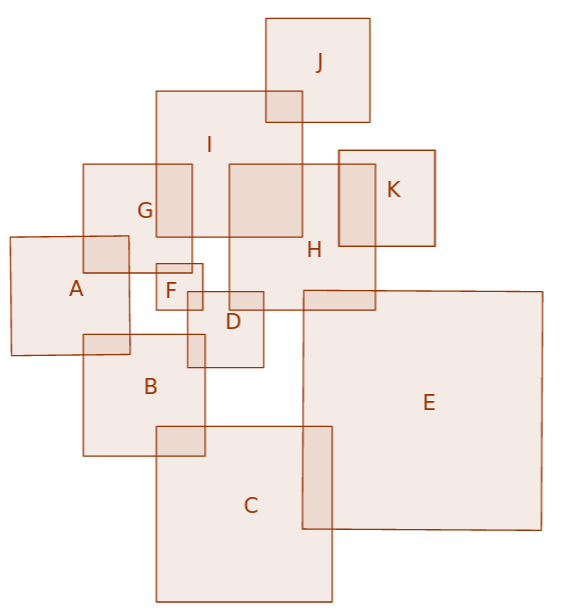
\includegraphics[scale=0.3]{tex_images/example_algorithm.png}  
    \caption{Example of application of the algorithm.}  
\end{figure}











\subsection{What about the other way?}


\begin{theorem}
    Every on-a-grid graph can be drawn as an intersection graph of squares. 
\end{theorem}



\begin{proof}
    Organize the squares by their order on RL parallel line; then from bottom to top. We denote them $v_{i,j}$. $i$ denotes on on which RL-parallel line they are;
    $j$ denotes the order (bottom-top) on the $i$-th line. \\
    The proof consists in an algorithm explaining how to construct the squares. It is done by considering the RL lines one by one. 
    
    Start by representing all the squares on the lowest RL-line. They have a default size of 2; when two vertex are neighbours, merge the corners and centers.
    When two vertices are not neighbours, merge their corners (Fig. 2). 
    \begin{figure}[h]
        \centering
        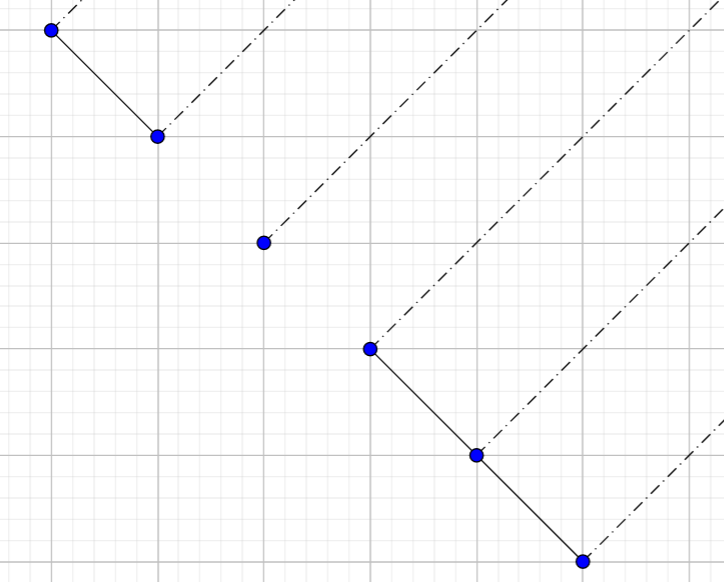
\includegraphics[scale=0.2]{tex_images/on_a_grid_2.png}
        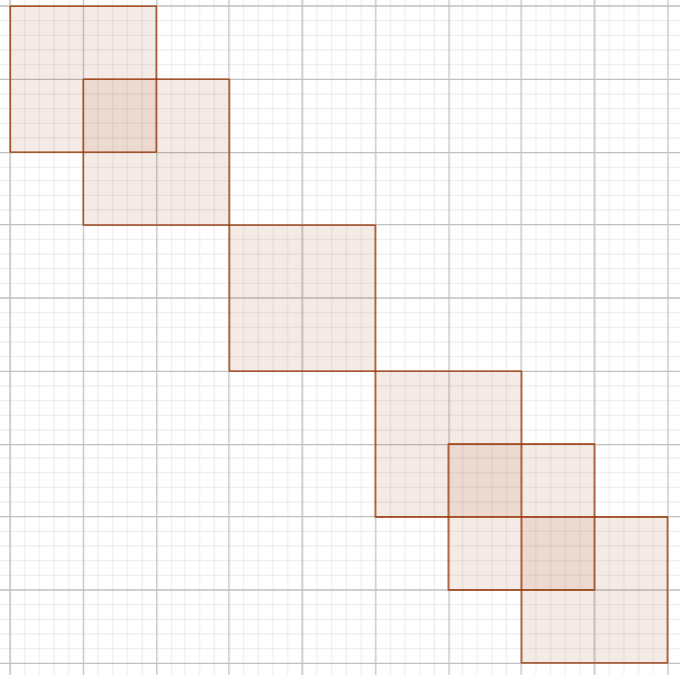
\includegraphics[scale=0.17]{tex_images/on_a_grid_3.png}
        \caption{Lowest RL diagonal treatment.}
    \end{figure}

    Now consider the next RL line. We can observe 4 different cases:
    \begin{itemize}
        \item a: The lines are identical.
        \item b: Some vertex of the previous have no neighbours here.
        \item c: Some vertex on the new line have no neighbours with the previous line.
        \item d: Mixes from b and c.
    \end{itemize}

    %n case of a: simply copy what has been done on the previous line and merge corners with centers accordingly.\\
    %In case of c: \\



\end{proof}

\end{document}